%----------------------------------------------------------------------------
\chapter{Experiments and results}\label{sect:Experiments}
%----------------------------------------------------------------------------
\section{Evaluation methods}

I used three methods to evaluate the results. The most basic method is the accuracy measure, which calculates the ratio of the correct answers as follows:

\[accuracy = \frac{correct\ answer}{all\ answer}\]

Since we are talking about graphs we need to measure the accuracy on the nodes and (if we are also training on them) the edges.
\[accuracy_{nodes\ and\ edges} = \frac{correct\ nodes + correct\ edges}{all\ nodes + all\ edges}\]

The other general evaluation metric in case of classification is the F-score. This is better for evaluating the results of a classification because it is not so greatly affected by the distribution of the classes. For this we need to calculate the true positive, true negative, false positive and false negative measures for every class. See on Figue~\ref{fig:TP_TN_FP_FN}.

\begin{figure}[!ht]
	\centering
	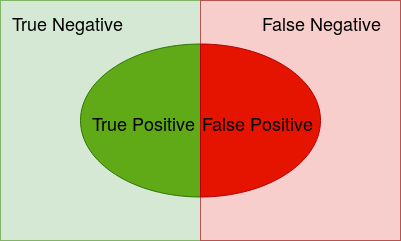
\includegraphics[width=100mm, keepaspectratio]{figures/F_score.png}
	\caption{The visual representation of the concept of true positive, true negative, false positive and false negative measures.}
	\label{fig:TP_TN_FP_FN}
\end{figure}


\[TP_{node==0} = number\ of\ correctly\ guessed\ node==0\]
\[TN_{node==0} = number\ of\ correctly\ guessed\ node!=0\]
\[FP_{node==0} = number\ of\ incorrectly\ guessed\ node==0\]
\[FN_{node==0} = number\ of\ incorrectly\ guessed\ node!=0\]

With these measures we can calculate the precision and recall. The precision tells us the ratio of correct guesses of the class out of every time the model predicted that class. The recall is the ratio of the correct guesses out of every instance that are actually in the class. The harmonic mean of the precision and recall is the F-score.

\[precision = \frac{TP}{TP + FN}\]
\[recall = \frac{TP}{TP + FP}\]

\[F1 = 2 * \frac{precision * recall}{precision + recall}\]

\subsection{ROUGE score}
The ROUGE score metric has been developed in 2004 by Chin-Yew Lin~\cite{ROUGE}. ROUGE is short for Recall-Oriented Understudy for Gisting Evaluation. The metric is used to determine the quality of a generated summary by comparing it to a human written summary.

ROUGE-N is the ROUGE measure over n-grams. An n-gram is an expression from the text with length n.
Since we only have one reference summary, the ROUGE-N score is as follows:

\[ROUGE-N = \frac{\sum_{n\_gram \in summary} Count_matching (n\_grams)}{\sum_{n\_gram \in summary} Count(n\_grams)}\]

Since the results are graphs and we need texts to calculate the ROUGE score, I restored the highest scoring sentences from the original article using a scoring system. This works quite simply, it averages the predictions of the nodes of a sentence, ignoring the stopwords.

\[score_{sentence} = \frac{\sum_{n \notin stopwords} n}{Count\ words\ without\ stopwords} \]

Using this score the sentences can be ordered by predicted relevance and the best four (like in the case of the extracted summary) can be chosen as the summary.

\section{Experiments}

At first I tried to get the Encode-Process-Decode model to predict whether to put something in the summary graph or not using only the word ids as features, but realized it would probably be more sufficient to also use the POS tags.

I also experimented with different loss functions, but for now i decided to use softmax cross entropy with output feature sizes of 2. This loss function is also available in the Appendices\ref{sect:Appendices}.

Besides the accuracy measurement, I also calculated the achieved precision, recall and F1-score on the test data to better understand the performance of the model.

\section{Results}
Training on more, than 7000 article for 5 epochs (Early stopping stopped it from running any longer) I've got the following results.
\begin{table}[!h]
	\centering
	\begin{tabular}{| c | c |}
		\hline
		Test loss & 0.4469867098715998 \\ \hline
		Correct test parts & 0.9584359204041673 \\ \hline
		Correctly solved test graphs & 0.0 \\ \hline
	\end{tabular}
	\caption{Softmax cross entropy loss and accuracy on the test set}
\end{table}

\begin{table}[!h]
	\centering
	\begin{tabular}{| c | c | c | c |}
		\hline
		 & precision & recall & f1 \\ \hline \hline
		edges0&0.959851063331886&1.0&0.9795142919687693  \\ \hline
		edges1 & 0.0 & 0.0 & 0.0 \\ \hline
		nodes0 & 0.9145702408368789 & 0.9852146581448155 & 0.9485789761340864 \\ \hline
		nodes1 & 0.6280412552891397 & 0.2133850485204265 & 0.3185415362603952 \\ \hline
	\end{tabular}
	\caption{The classification report on the test set}
\end{table}

As it is clear from this the network hardly ever classifies a node as "1", meaning that is should be in the summary graph, but when it does it is 62.8\% accurate.

\subsection{Example}
To better visualize the results I've taken an example of the expected (Figure~\ref{fig:expected}) and the calculated graphs (Figure~\ref{fig:calculated})

\begin{figure}[!ht]
	\centering
	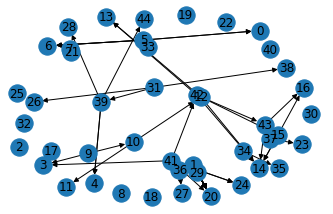
\includegraphics[width=75mm, keepaspectratio]{figures/expected.png}
	\caption{Expected graph with just the nodes and edges labeled 1.}
	\label{fig:expected}
\end{figure}

\begin{figure}[!ht]
	\centering
	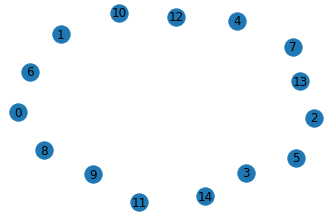
\includegraphics[width=75mm, keepaspectratio]{figures/calculated.png}
	\caption{Calculated graph with just the nodes and edges labeled 1.}
	\label{fig:calculated}
\end{figure}

As it is shown, the method is very conservative about choosing the nodes, and even more so with the edges. The reason for this might be the few number of edges labeled 1 in the target graph.